% !TEX encoding = UTF-8 Unicode

% This is a simple template for a LaTeX document using the "article" class.
% See "book", "report", "letter" for other types of document.
 
\documentclass[12pt]{article} 

%%% PACKAGES
\usepackage[utf8]{inputenc} % set input encoding (not needed with XeLaTeX)
\usepackage[letterpaper,top=0.65in,bottom=0.7in,left=0.75in,right=0.75in]{geometry}
\usepackage{graphicx}
\usepackage{tikz}
\usepackage{tikzrput}
\usepackage{lipsum}
\usepackage{psvectorian}
\usepackage{pgfornament}
\usepackage{fontspec} \setmainfont{Garamond}
\usepackage[parfill]{parskip} % Activate to begin paragraphs with an empty line rather than an indent
% \usepackage{background}
\usepackage{varwidth} 
\usepackage{lettrine}
\usepackage{parcolumns}
% \usepackage{amsmath}
% \usepackage{pbox} 
\usetikzlibrary{calc}
\pagestyle{empty}
% \parindent=0pt
\usepackage{multicol}

% \newfontface\applechanceryfont{Apple Chancery}


\def\fontASize{48}
\newcommand{\fontA}{\fontsize{\fontASize}{\fontASize}\fontspec{Garamond}}
% \newcommand{\fontACursive}{\fontsize{\fontASize}{\fontASize}\applechanceryfont}


\def\fontBSize{28}
\newcommand{\fontB}{\fontsize{\fontBSize}{\fontBSize}\fontspec{Garamond}}
% \newcommand{\fontBCursive}{\fontsize{\fontBSize}{\fontBSize}\applechanceryfont}


\def\fontCSize{32}
\newcommand{\fontC}{\fontsize{\fontCSize}{\fontCSize}\fontspec{Garamond}}
% \newcommand{\fontCCursive}{\fontsize{\fontCSize}{\fontCSize}\applechanceryfont}


\def\fontDSize{18}
\newcommand{\fontD}{\fontsize{\fontDSize}{\fontDSize}\fontspec{Garamond}}
% \newcommand{\fontDCursive}{\fontsize{\fontDSize}{\fontDSize}\applechanceryfont}

\def\fontESize{12}
\newcommand{\fontE}{\fontsize{\fontESize}{\fontESize}\fontspec{Garamond}}
% \newcommand{\fontECursive}{\fontsize{\fontESize}{\fontESize}\applechanceryfont}

\def\fontFSize{8}
\newcommand{\fontF}{\fontsize{\fontFSize}{\fontFSize}\fontspec{Garamond}}
% \newcommand{\fontECursive}{\fontsize{\fontESize}{\fontESize}\applechanceryfont}


\date{}
\title{}
\author{}


% %%% HEADERS & FOOTERS
% \usepackage{fancyhdr} % This should be set AFTER setting up the page geometry
% \pagestyle{fancy} % options: empty , plain , fancy
% \renewcommand{\headrulewidth}{0pt} % customise the layout...
% \lhead{\fontD{}www.meridianensemble.net}\chead{}\rhead{\fontD{}info@meridianensemble.net}
% \lfoot{}\cfoot{}\rfoot{}






\title{}
\begin{document}%
%%% BORDER:
% \vbox to 0pt{{\hbox{ABCD}}}\vskip 0pt}\parskip=0pt%
%
% \makebox[0pt]{\vbox to 0pt{
    % % \hbox{AHOY}
    % \hbox to 0pt{%
        % \hskip 0in%
        % \vbox to 0pt {%
            % \vskip 5in%
            % % \pgfornament[height=1.8in]{160}%
                % % \makebox[\hsize][c]{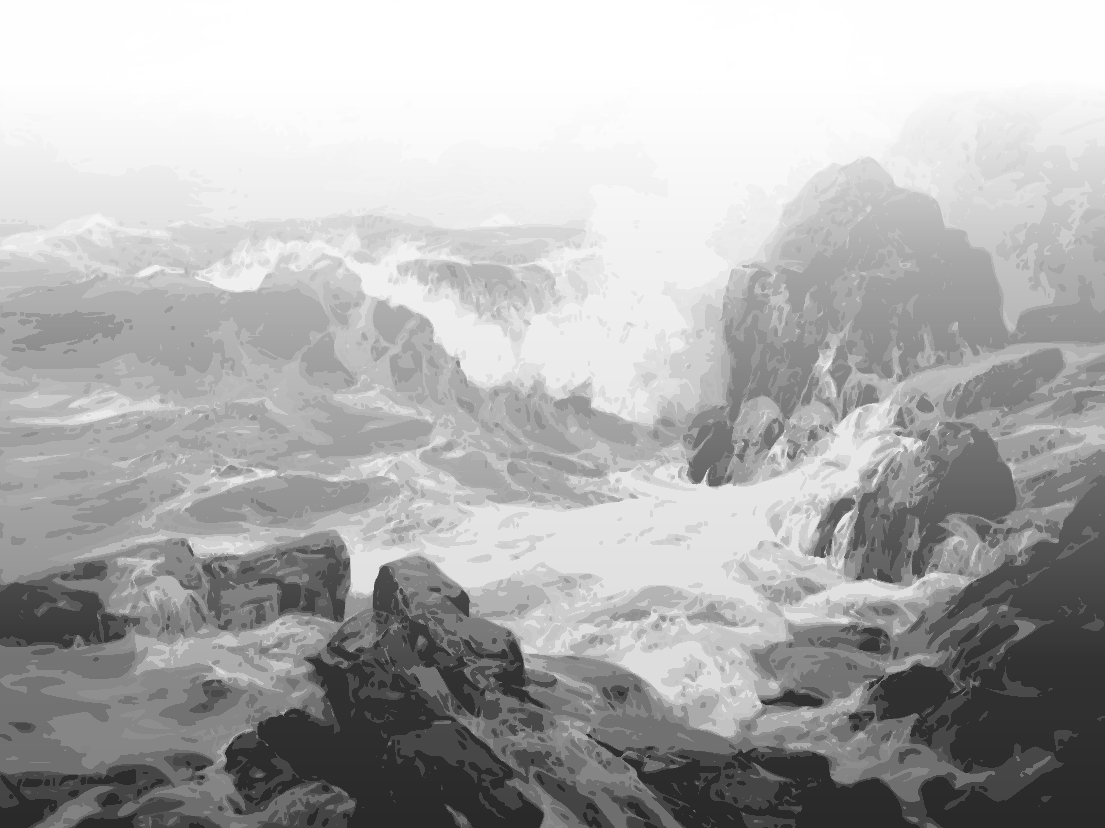
\includegraphics[trim= 0mm 0mm 0mm 60mm, width=8in, height=10in, clip]{page-decoration.pdf}}
            % \vfilneg
        % }%
    % }%
    % % \relax
    % \hrule height0pt width0pt depth0pt %the depth of our vbox will be the same as the depth of the last element in the vbox, so we make that zero
    % \vfilneg%
% }}%
\begin{tikzpicture}[overlay,remember picture]
    \draw [line width=3pt,rounded corners=15pt,double]
        ($ (current page.north west) + (0.43in,-0.55in) $)
        rectangle
        ($ (current page.south east) + (-0.43in,0.55in) $);
\end{tikzpicture}%
%
% \hbox to \hsize{
    % \hfill
    % \vbox to 1.2in{%
        % \vfill%
        % \hbox{\pgfornament[height=2.3in]{160}}
    % }%
% }
% \vtop to 0pt{\vbox to 0pt{\vtop to 0pt{\hbox{ABCD}}}}%
\vskip -0.1in%
\edef\originalParskip{\the\parskip}%
% \hbox to 0pt%
  % {%
  	% \vbox to 0pt {ABCD}	%
  	% \hss%
  % }\relax%
\hbox to \hsize{%
    \begin{varwidth}{3in}%
        % \parskip=0pt%
        \noindent\raggedright\fontE{}\textbf{Saturday, November 23, 7:00 PM}\vskip 0.02in%
        Magnolia United Church of Christ\linebreak%
        3555 West McGraw Street\linebreak%
        Seattle, WA%
    \end{varwidth}
    \hfil
    \begin{varwidth}{3in}%
        % \parskip=0pt%
        \noindent\raggedright\fontE{}\textbf{Sunday, November 24, 2:00 PM}\vskip 0.02in%
        Saint Clement's Episcopal Church\linebreak%
        1501 32nd Avenue South\linebreak%
        Seattle, WA%
    \end{varwidth}%
}
% \vskip 0.1in%
% \hrule%
\vskip 1.5in
{\centering
    \fontA{}MERIDIAN ENSEMBLE
    \vskip 0in
    \fontB{}presents
    \vskip 0.3in
    % \rput[r](-3pt,3pt){\pgfornament[scale=.45]{72}}
    \fontA{}The Gravity of Beauty%
    % \rput[l](3pt,3pt){\pgfornament[scale=.45]{73}}\\
    % \rput(0,0){\pgfornament[scale=.5]{85}}
    \vskip 0.15in
}%
\hbox to \hsize{%
    \hfill%
    \vbox{\hsize=6.6in
        \begin{center}
        \lineskip=5pt
        \fontD{}An exploration of secular choral repertoire from pre-revolutionary Russia (Kalinnikov, Arensky, Kui, Glazunov, Rachmaninov) featuring a few gems by fellow European masters (Saint-Saens, Elgar, Brahms, Reger)%
        % \vskip 0.2in
        % \fontB{}Passionately sung by 15 chamber singers    
        \end{center}%
    }%
    \hfill%
}%
%
% \vskip 0.2in
% \hrule
\vfil
\hbox to \hsize{%
    % \hbox to 0pt{%
        % \hskip 0in%
        % \vbox to 0pt {%
            % \vskip -9in%
            % % \pgfornament[height=1.8in]{160}%
            % \fbox{%
                % \makebox[\hsize][c]{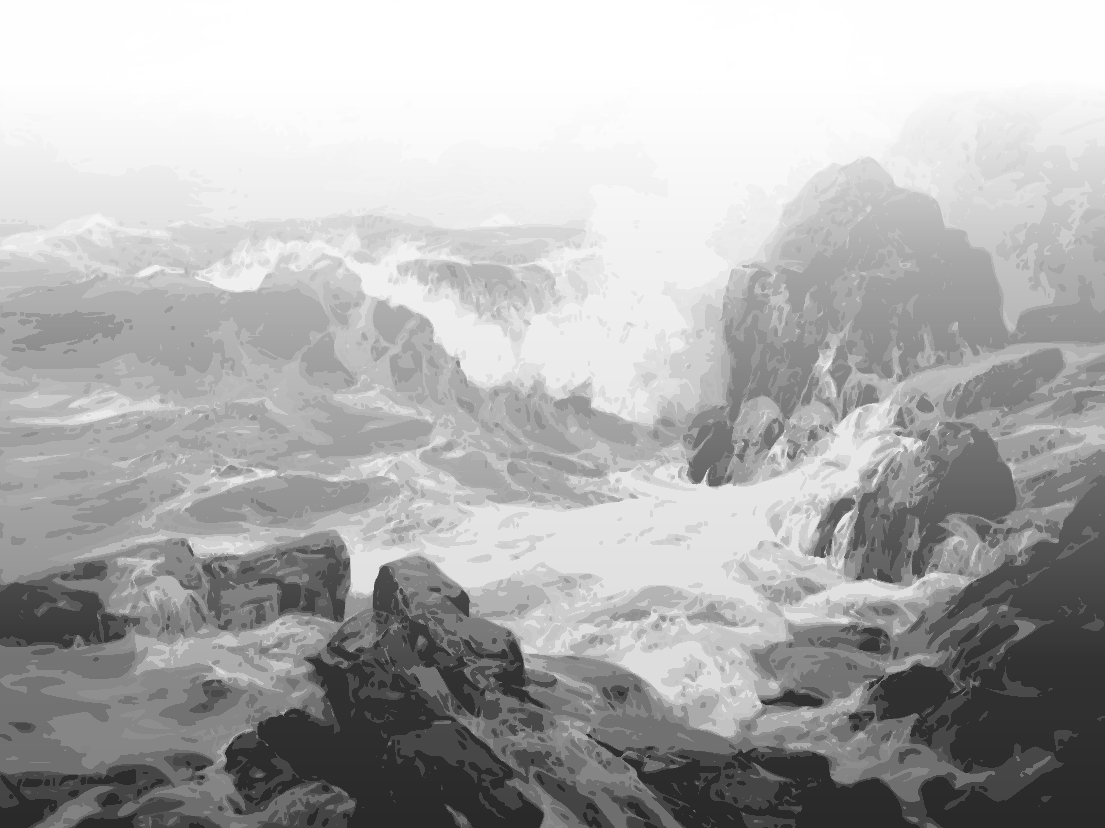
\includegraphics[trim= 0mm 0mm 0mm 60mm, width=8in, height=10in, clip]{page-decoration.pdf}}
             % }%
            % \vfilneg
        % }%
    % }%
    % \fbox{\begin{varwidth}[b]{8in}%
        % \pgfornament[height=2.3in]{160}%
        % \vskip 0pt
        % \hbox{}
        % % \hrule height10pt width20pt depth0pt\relax\hss\relax\unskip\hskip 0pt minus 1fill %
    % \end{varwidth}}
    \hfil%
    % \begin{minipage}[b]{4.3in}\setlength{\parskip}{\medskipamount}
        % % \hrule height2pt
        % {\fontD{}\textbf{Dear Friends,}}
        % \bigskip
        % \lettrine[lines=2,loversize=0.25,findent=-2pt]{I}{} am beyond delighted to present Meridian Ensemble and our Songs of Passion. In this
        % program we explore Passion and a special thrill that makes it such a powerful emotion.
        % A state of intense, burning desire, Passion can be a trigger of incredible, fantastic
        % accomplishments; it can also leave one scarred so deeply and longing to heal so
        % desperately. From overcoming hate and setting oneself on the path of love, from
        % rediscovering one’s voice and bursting in a new song, from separation by distance and
        % time to long-awaited reunion of the loved ones, \makebox{Meridian Ensemble} is excited to share
        % with you a myriad of expressions of Passion through the beauty of chamber choral
        % performance.

        % \bigskip\raggedright
        % Sincerely,\vskip 0.04in
        % % Yuly Kopkin,\linebreak
        % % Artistic Director
        % {\fontD{}\textbf{Yuly Kopkin,
        % Artistic Director}}
    % \end{minipage}%
    \hfil
}%
\vskip 0.05in%
\pagebreak
\vbox to \vsize {
\vfil
\hbox to \hsize{
\hfil%
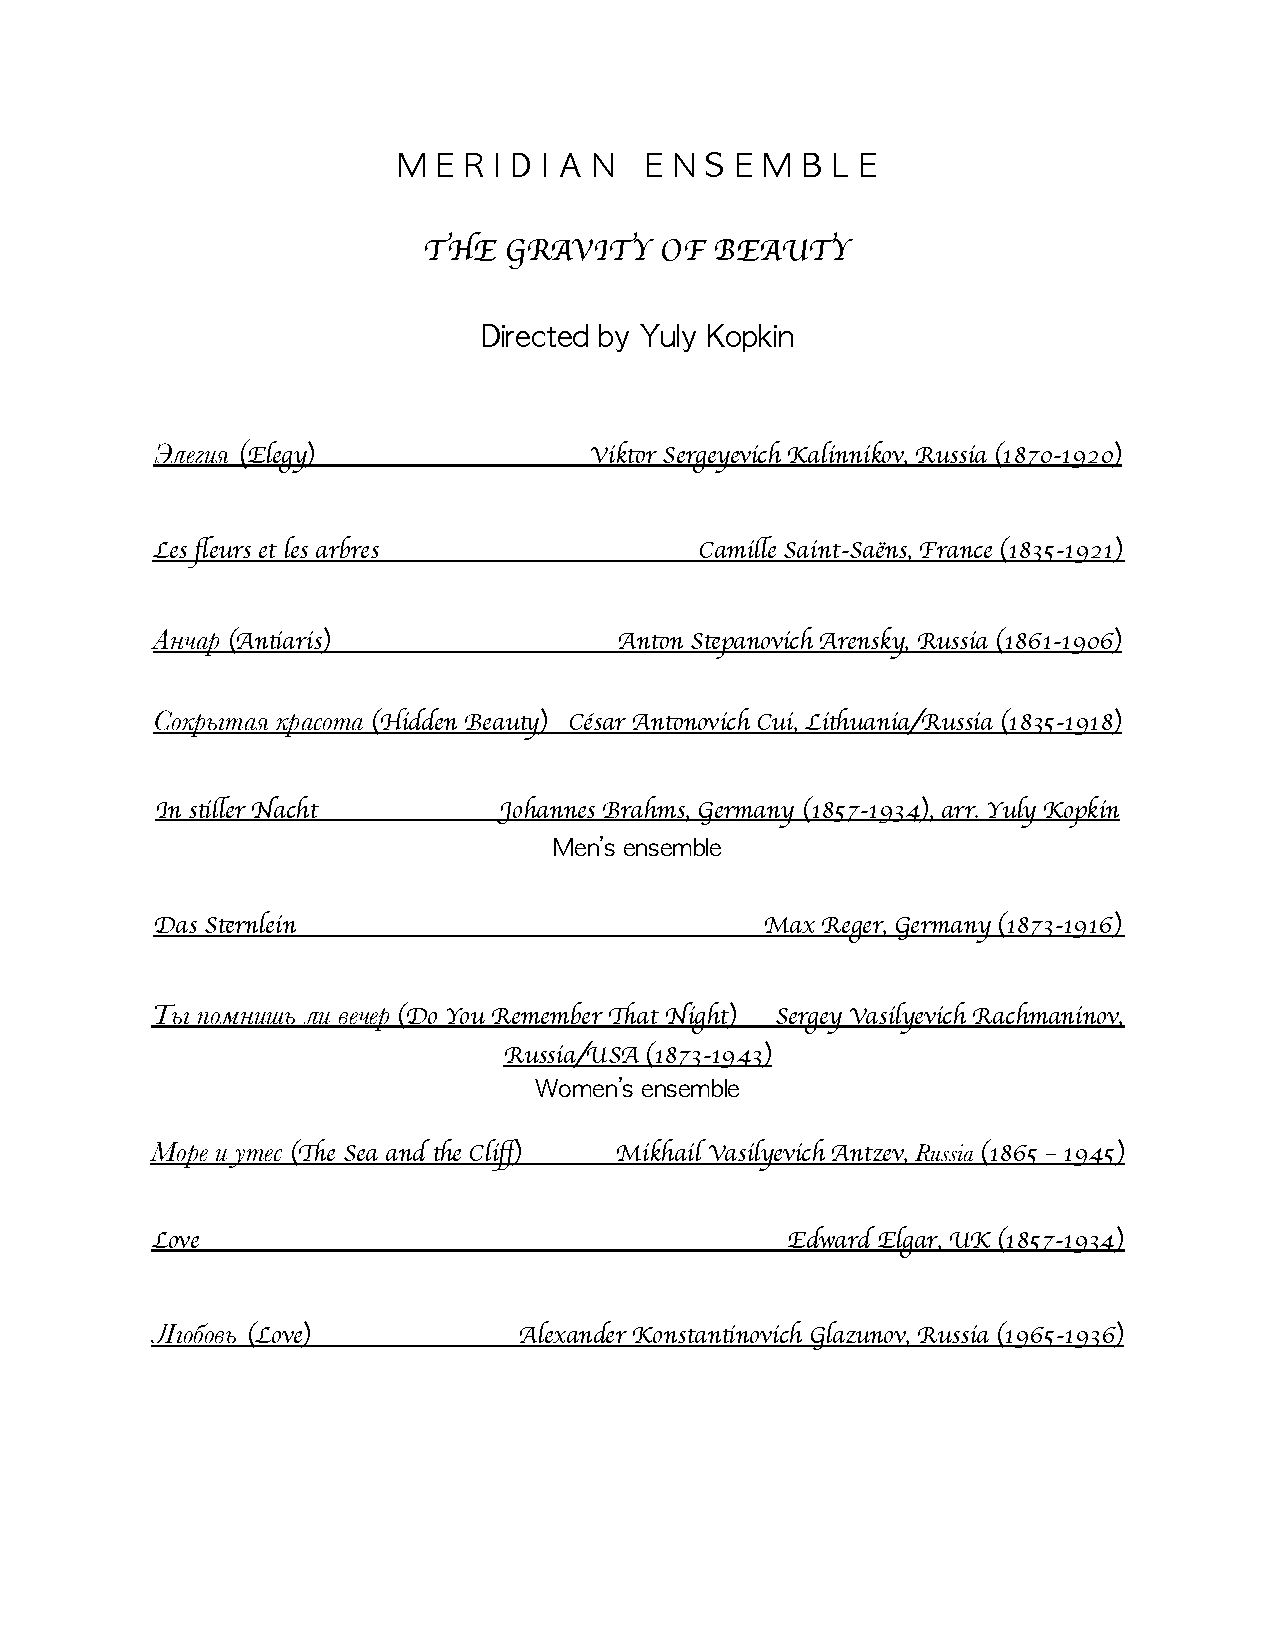
\includegraphics[page=1,natheight=11in,natwidth=8.5in,trim=1in 1in 1in 1in]{pdfs-to-include/ProgramTitles.pdf}%
\hfil%
}%
\vfil
}
\pagebreak
\vbox to \vsize {\raggedright
\begin{multicols}{2}
\raggedright%
\vbox{
\fontF{}\noindent ELEGY (by Pushkin)

The flying chain of clouds is thinning in the sky.\linebreak{}
O you, the Evening Star, the star of woe on high,\linebreak{}
Your beam is silvering the distant withered plains,\linebreak{}
And both the dreamy bay, and murky rocky chains.

I love your vague glow there in the heavenly height;\linebreak{}
And all my sleepy thoughts were woken by your light.\linebreak{}
I do remember you, o star how you were rising,\linebreak{}
Above the peaceful land where everything was pleasing,

Where slender poplars raised their crowns above the dales,\linebreak{}
Where tender myrtles slept and cypress in dark veils,\linebreak{}
Where in the middle of day the songs of waves were haunting.\linebreak{}
Long time ago when I was there upon the mountain\linebreak{}
Above the sea I dragged my thoughtful laziness.\linebreak{}
}
\vskip\parskip
\vskip\parskip
\vbox{
\fontF{}\noindent LOVE (by Jukovsky)

By the nature’s will\linebreak{}
On the fragrant meadow\linebreak{}
In the flowering valley\linebreak{}
And in the lush chamber\linebreak{}
And in the starry sparkling of silent nights\linebreak{}
I only breathe you.

Deep sweetness\linebreak{}
Deep flame you pour in me.

In the life-affirming spring,\linebreak{}
In the incense of flowers\linebreak{}
You embrace me with the calmness of the sky,
Holy love! %
}
\vskip\parskip
\vskip\parskip
\vbox{
\fontF{}\noindent ARENSKY - ANCHAR (by Pushkin)

In desert, withered and burned,\linebreak{}
On ground that is dry and sultry,\linebreak{}
Anchar, alone in the world,\linebreak{}
Stands like an awful, silent sentry.

The nature of the thirsty land,\linebreak{}
Has borne him on the day of terror,\linebreak{}
And flesh of roots and boughs, dead,\linebreak{}
Was filled with venom blood forever.

The poison oozes through his bark\linebreak{}
And melts at noon in beams from heaven,\linebreak{}
And thickens in the evening dark--\linebreak{}
A tar, transparent one and heavy.\linebreak{}
And birds don't visit him at all,\linebreak{}
Not any tiger for him wishes\linebreak{}
And only, sometimes, comes a whirl,\linebreak{}
To fly away, but as pernicious.

And if, by chance, a cloud sprays\linebreak{}
His leaves in wandering alone,\linebreak{}
From all his twigs, the poisoned rains\linebreak{}
Pour into scorching sand and stone.\linebreak{}
But once a man had sent a man,\linebreak{}
To desert -- to the poison demon,\linebreak{}
The slave obediently ran,\linebreak{}
And by the morn he brought the venom.

He brought the resin of the death,\linebreak{}
A twig with faded leaves, by morning,\linebreak{}
And heavy sweat, on his pale face,\linebreak{}
In icy rivulets was rolling.

He came, and lay, and fell in fit,\linebreak{}
In shadow of the tent, in fluster,\linebreak{}
The slave had died by the feet\linebreak{}
Of his inexorable master.

The prince immediately breathed\linebreak{}
The evil tar into his arrows,\linebreak{}
And sent with them the poison-death,\linebreak{}
To alien lands--the lands of neighbors.
}
\vskip\parskip
\vskip\parskip
\vbox{
\fontF{}\noindent THE SEA AND THE CLIFF (by Tutchev)

Raging, seething,\linebreak{}
lashing, whistling, roaring,\linebreak{}
leaping for the skies,\linebreak{}
the unassailable skies…\linebreak{}
Is it hell, some hellish force\linebreak{}
beneath the boiling cauldron\linebreak{}
churning up the deeps,\linebreak{}
some hellish fire\linebreak{}
turning the sea-world upside down?

Frenzied wave-onslaught…\linebreak{}
Nothing stops it, nothing can…\linebreak{}
Roars, whistles, screams, howls…\linebreak{}
Smashing cliffs along the coast…\linebreak{}
Peaceful, haughty,\linebreak{}
unmoved by the clowning sea,\linebreak{}
motionless, changeless,\linebreak{}
born at creation, you stand, our titan!

Battle-maddened,\linebreak{}
leaping into fateful struggle\linebreak{}
waves come howling back\linebreak{}
to beat against your granite face…\linebreak{}
The changeless stone\linebreak{}
dashes aside the noisy onslaught.\linebreak{}
Scattered waters fall apart.

Impotent gusts fall grumbling away.\linebreak{}
Stand, mighty cliff!\linebreak{}
Just wait awhile.\linebreak{}
The thundering waves will tire\linebreak{}
of warring with your foot.\linebreak{}
Exhausted by its spiteful game\linebreak{}
the sea will be subdued.\linebreak{}
Forget this howling affray.\linebreak{}
Beneath the foot of the titan,\linebreak{}
the waves will slink away.%
}
\vskip\parskip
\vskip\parskip
\vbox{
\fontF{}\noindent LES FLEURS ET LES ARBRES

The flowers and the trees,\linebreak{}
The bronzes, the marbles,\linebreak{}
The golds, the enamels,\linebreak{}
The sea, the waterfalls,\linebreak{}
The mountains and the plains\linebreak{}
Console our pain.

Eternal nature,\linebreak{}
You seem more beautiful\linebreak{}
To a heart in sorrow,\linebreak{}
And art reigns over us,\linebreak{}
Its flame illuminates\linebreak{}
the laughter and tears. 
}
\vskip\parskip
\vskip\parskip
\vbox{
\fontF{}\noindent DAS STERNLEIN

There was a star in the sky,\linebreak{}
A star of good kind;\linebreak{}
It seems so lovely,\linebreak{}
So lovely and so tender!

I knew his place\linebreak{}
In the sky where it stood;\linebreak{}
He went to the threshold in the evening\linebreak{}
And searched until I found it.

And stopped for a long time,\linebreak{}
I had great joy in me:\linebreak{}
To look at the star;\linebreak{}
And thanked God for that.

The star has disappeared;\linebreak{}
I’m looking back and forth\linebreak{}
Where I once found it,\linebreak{}
And do not find it anymore.
}

% \vskip\parskip
% \vskip\parskip
% \vbox{
% \fontF{}\noindent LES FLEURS ET LES ARBRES

% The flowers and the trees,\linebreak{}
% The bronzes, the marbles,\linebreak{}
% The golds, the enamels,\linebreak{}
% The sea, the waterfalls,\linebreak{}
% The mountains and the plains\linebreak{}
% Console our pain.

% Eternal nature,\linebreak{}
% You seem more beautiful\linebreak{}
% To a heart in sorrow,\linebreak{}
% And art reigns over us,\linebreak{}
% Its flame illuminates\linebreak{}
% the laughter and tears. 
% }
% \vskip\parskip
% \vskip\parskip
\vfill
\vfill
\end{multicols}






\vfil
\hbox to \hsize{
\hfil%
% \includegraphics[page=2,natheight=11in,natwidth=8.5in,trim=1in 1in 1in 1in]{ProgramTitles.pdf}%
\hfil%
}%
\vfil
}
\pagebreak
\vbox to \vsize {
\vfil
\hbox to \hsize{
\hfil%
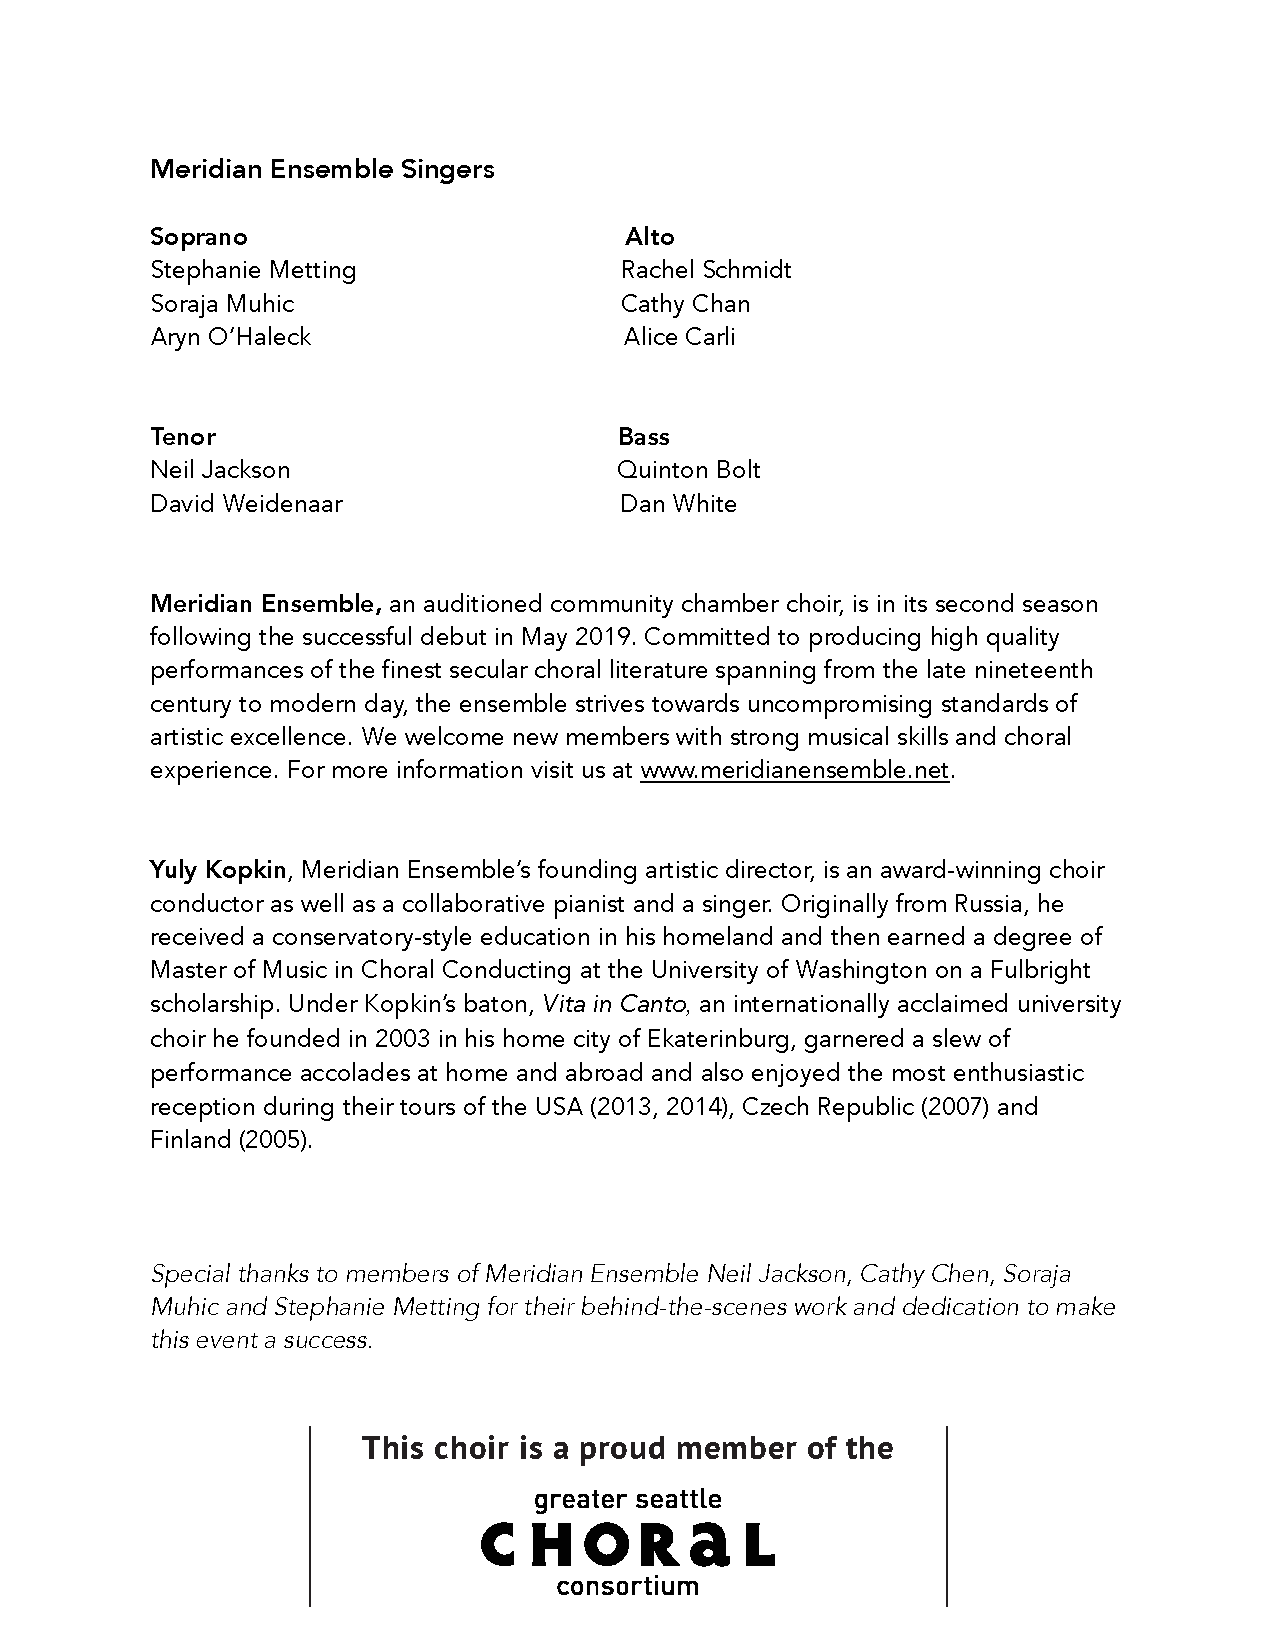
\includegraphics[page=1,natheight=11in,natwidth=8.5in,trim=1in 1in 1in 1in]{pdfs-to-include/About-ensemble-and-director.pdf}%
\hfil%
}%
\vfil
}

% {\centering
    % \fontB{}MERIDIAN ENSEMBLE
    % \vskip 0.2in
    % % \rput[r](-3pt,3pt){\pgfornament[scale=.45]{72}}
    % \fontB{}Songs of Passion%
    % % \rput[l](3pt,3pt){\pgfornament[scale=.45]{73}}\\
    % \vskip 0.4in
    % \fontB{}Directed by Yuly Kopkin%
    % \vskip 0.4in
% }%

% My Spirit Sang All Day\dotfill{}Gerald Finzi, UK (1901\textendash1956)\linebreak

% \bigskip

% I Had No Time To Hate\dotfill{}Nathan Howe, USA (1982\textendash\ )\linebreak

% \bigskip

% Нам звезды кроткие сияли\dotfill{}Viktor Kalinnikov, Russia (1870\textendash1927)\linebreak
% (Nam zyvozdy krotkiye siyali)

% \begin{parcolumns}[rulebetween=true]{2}
% \raggedright%
% \colchunk{Nam zvyozdy krotkiye siyali, chut’ veyal tikhiy veterok.  Krugom tzvety blagauhali, i volny laskovo sheptali u nashikh nok.\vskip\parskip}
% \colchunk{The distant stars shone for us, all around us the blossom of flowers smelled so sweetly,\linebreak{}And the waves whispered gently at our feet.\vskip\parskip}
% \colplacechunks
% \colchunk{this is chunk 2 in column 1}
% \colchunk{this is chunk 2 in column 2}
% \colplacechunks


% \end{parcolumns}



\end{document}